\documentclass{article}%
\usepackage[T1]{fontenc}%
\usepackage[utf8]{inputenc}%
\usepackage{lmodern}%
\usepackage{textcomp}%
\usepackage{lastpage}%
\usepackage{authblk}%
\usepackage{graphicx}%
%
\title{MKP{-}1 regulates cytokine mRNA stability through selectively modulation subcellular translocation of AUF1}%
\author{Nathan Bradley}%
\affil{Nephrology Unit, Department of Medicine, Faculty of Medicine, Thammasat University (Rangsit Campus), Khlong Nueng, Khlong Luang, Pathum Thani 12121, Thailand}%
\date{01{-}01{-}2004}%
%
\begin{document}%
\normalsize%
\maketitle%
\section{Abstract}%
\label{sec:Abstract}%
On December 19, 2003, researchers at the Johns Hopkins University School of Medicine conducted a research study that reveals the link between the adrenal gland and NaC{-}KCATPase activity in all myocytes, the bodys cells responsible for a variety of vital health processes. In this study, they tested the function of molecules used to detect proteins in the immune system.\newline%
The researchers created {-}catenin, an immunoglobulin that binds to mRNA in the messenger RNA, a compound that assists in identifying specific proteins in cells language. In one experiment, they found that as {-}catenin binds to the mRNA, it produces a a key signal that redetermines the development of different kinds of protein. (For a full description of the research, see NaC{-}KCATPase Activity in Myocytes, on Page 4 .)\newline%
In other recent research, the researchers identified an inborn inflammation mechanism in the atherosclerotic cardiovascular heart. Recent research has established that the inflammatory state is ultimately a type of debility, not caused by kidney stones and possibly related to pre{-}existing cardiovascular disease, arthritis, or a known inflammation of the autonomic nervous system in the body.\newline%
By demonstrating the impact of drug{-}based medications on the response to chronic inflammation and inflammation{-}related factors in all myocytes, researchers hope to identify avenues for the treatment of type 2 diabetes, heart failure, hypertrophic cardiomyopathy, diabetes mellitus, atherosclerosis, or chronic pain.

%
\subsection{Image Analysis}%
\label{subsec:ImageAnalysis}%


\begin{figure}[h!]%
\centering%
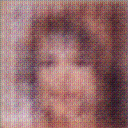
\includegraphics[width=150px]{500_fake_images/samples_5_426.png}%
\caption{A Man Wearing A Black Jacket And A Black Cat}%
\end{figure}

%
\end{document}